\chapter{Conclusion}
It has been postulated that microbiota associated with multicellular organisms act as second genomes for their hosts \cite{grice2012human}. That is, the collective genomes of the microorganisms within a microbiome provide functions that are not encoded within the host organism’s genome. Indeed, many parallels can be drawn between the genome of the host and the composition of the microbiota. The host’s genome and microbiota are both structured into individual, non-overlapping units where the genome contains genes and the microbiota contains individual microbial taxa. Each unit within the genome and microbiota can be “expressed” at different levels depending on various environmental stimuli where genes are transcribed into mRNA of different abundances and individual microbial taxa multiply to have different cell counts. Moreover, trans-regulation occurs in both gene expression and microbial cell pro{}liferation. For instance, gene x may regulate the expression of gene y through binding to its promoter and microbe a may regulate the proliferation of microbe b by providing it critical nutrients. A striking difference between the innate genome and the second genome, however, is the nature by which they are acquired. Genomes are hereditary, being passed along from parent to offspring. A microbiota, however, is acquired from the environment. In the case of a plant, the root microbiota is primarily derived from the soil \cite{Zarraonaindia2015}. Characterizing the contents of the plant’s second genome and understanding the rules governing its acquisition are the primary foci of this dissertation.

\section{Chapter 1}
In the first chapter, I described the general characteristics of rice root-associated microbiota. We began by quantifying how microbial community profiles differ as a function of distance to the root. We detailed the microbiota within three root-associated compartments: the rhizosphere (soil tightly adhering to the root), the rhizoplane (the root surface), and the endosphere (the interior of the root). We found all three of these compartments to host distinct microbial communities and that each community is also distinct from the microbiota of unplanted soil. The rhizoplane and endosphere communities had lower microbial diversity compared to the rhizosphere and bulk soil, suggesting that there is a niche specialization for the microbiota in these root-associated compartments. We next characterized the effect of soil type on the root-associated microbial communities of rice. We found that soil originating from various rice fields host distinct sets of microbes and this in turn determines the subset of microbes that can colonize the roots of plants growing within these soils. We found similar trends in the trends in the abundance of various phyla across the root-associated compartments of plants grown in the different soils. For instance, in each soil Acidobacteria microbes have a decreasing abundance from the soil to the inside of the root, while Proteobacteria have an increased abundance inside the root and lower abundance in the soil. We also found that soil communities can be affected by agricultural practice. Specifically, root-associated microbiota are differentiable based upon whether the plants were grown under organic or conventional cultivation. We next characterized how the microbiota differs between various domesticated rice varieties. We profiled the microbiota from several cultivated varieties of two domesticated rice species, \textit{Oryza sativa} and \textit{Oryza glaberrima}, and found that rice genotype has a very minimal (although significant) effect on the root-associated microbiota. Many of these results have been corroborated by similar studies in other plant models. The results of the experiments are summarized in the visual model below. The model can be interpreted as such:
\begin{itemize}
\item Different soils host different consortia of microbes which can depend on geography or agricultural practice. This is indicated by different colors between the soil microbiota in the model.
\item Rice plants assemble a root-associated microbiota from the soil in which the plants are growing and this microbiota resembles the parent soil. The microbes that assemble on the inside of the root are much reduced subset of the soil community. This is indicated by the lighter color within the circle of the root-associated microbiota in the model.
\item Rice genotype has only a small effect on the root-associated microbiota even though much visible phenotypic diversity exists between the varieties. In the model, this is portrayed as the different hues in color between the different varieties. Please note that they are still reminiscent of the original hue of the parent soil in which the plants are growing.
\end{itemize}

\begin{figure}[h]
\centering
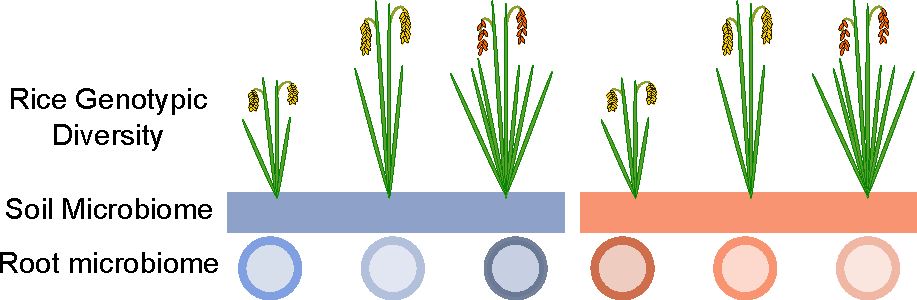
\includegraphics[width=5in]{Figures/figurec_1}
\caption[Figure 5.1]{\textbf{Model depicting host and environmental factos affecting the root-associated microbiota}}
\label{Figure 5.1}
\end{figure}

\section{Chapter 2}
In the second chapter, I characterized how the rice root-associated microbiota differs from other plants' microbiotas. We were perplexed that genotypic variation within two species of the Oryza genus only had a small impact on the root-associated microbiota. The varieties that we used for our experiment had distinct morphological traits that made each variety easily identifiable, yet their root microbiota was overall remarkably similar. We hypothesized perhaps there was a large conservation of root-associated microbiota across different lineages of flowering plants. We tested this hypothesis by first compiling published data from other plant root-associated microbiota studies that used similar methods to the methods in my first chapter. We found that each plant species assembles a distinct microbiota, but that his effect is confounded by the studies occurring in different geographic regions and environments. The rice microbiota was an outlier in this analysis, potentially due to its semi-submerged growth habit. We therefore collected and analyzed the root-associated microbiotas of three separate host plants growing in the same semi-submerged conditions as rice. We found that the microbiota from these plants, all of which are common rice paddy weeds with broad distributions across the United States, have distinct sets of microbial taxa colonizing their root-associated compartments. Rice, however, hosted an outlier microbiota compared to the other plants. The microbiota of rice plants were enriched for methane-producing microbes while the other plant species hosted microbiotas enriched for methane-utilizing microbes. It was also found from this experiment that the rice rhizosphere microbiota composition is notably similar to the microbiota from unplanted agricultural soil. We attributed this effect to continuous and intensive cultivation of rice which may in turn ``domesticate'' the soil microbiota to be more like the rhizosphere microbiota from rice. I have summarized the results of this analysis in the visual model below:

\begin{itemize}
\item The composition of the soil microbiota in which the different host plants are growing is represented by the orange box.
\item Each species assembled a significantly different microbiota as represented by the different colors of the root-associated microbiota circles for each host species. Notice that the different rice genotypes host a microbiota that is more similar to the hue of the bulk soil than the microbiotas of the other included host plant species.
\item The differences in microbiota composition between the different host species may have functional and environmental impacts, illustrated by the finding that the rice plants host more methanogenic microbes than the other host species in the same field.
\end{itemize}

\begin{figure}[h]
\centering
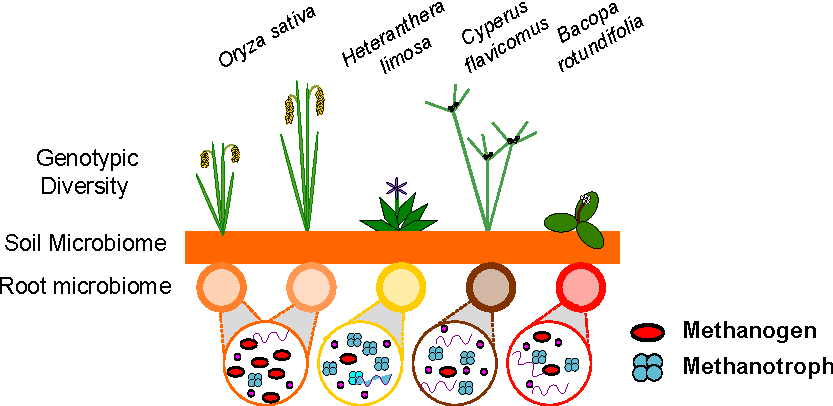
\includegraphics[width=6in]{Figures/figurec_2}
\caption[Figure 5.2]{\textbf{Model depicting the impact of host plant genotypic diversity on the root-associated microbiota}}
\label{Figure 5.2}
\end{figure}

\section{Chapter 3}
In the third chapter, I characterized how the root-associated microbiota changes throughout the lifecycle of the rice plant. Plants undergo large morphological and physiological shifts throughout their life cycle which in turn have stage-specific nutritional and environmental demands \cite{Ishimaru2013}. We sampled the microbiota of rice plants growing in single field in California over the course of three seasons. Remarkably, we found there to be only a small amount of variation across the seasons. In each compartment, we found that the microbiota progressively shifts throughout the growing season, especially during the vegetative phase of growth. These shifts are most pronounced in decreasing abundance of Betaproteobacteria and increasing abundance of Deltaproteobacteria over the course of the season. Upon the entry into the reproductive stage of development, we found that the overall composition of root-associated microbiota stabilizes. This shift appeared to be faster in the endosphere and rhizoplane than in the rhizosphere. In the first two seasons of our experiment, we were unable to definitively attribute the shifting microbiota to plant developmental progression in the first two seasons of our trial because all of the sampled plants were synchronized for developmental progression. There are environmental and edaphic factors that fluctuate over the season and there is also a possibility that the microbes require a certain amount of time to stabilize independent of plant developmental stage. To examine the effect of plant developmental stage on the root-associated microbiota independent of plant age and fluctuating environmental and edaphic factors, we grew different varieties that progress through development at different rates. Indeed, we found that faster progressing genotypes had faster shifting microbiotas. By using a machine learning approach, we were able to identify individual microbes whose abundance are descriptive of developmental stage. I have summarized our model for root-associated microbiota shifts over the lifecycle of the rice plant in a visual model below.

\begin{itemize}
\item The microbiota shifts in a gradient over the course of the season as mimicked by the hue of the horizontal bar shifting from the beginning of the season to the end.
\item The microbiota shifts during the vegetative phase of the rice plant's life (i.e. the seedling and tillering stages) until the onset of reproduction where the microbiome remains relatively steady. This pattern is denoted by the shifting hue of the horizontal bar during the vegetative phase which becomes steady at the onset of the panicle initiation stage.
\end{itemize}

\begin{figure}[h]
\centering
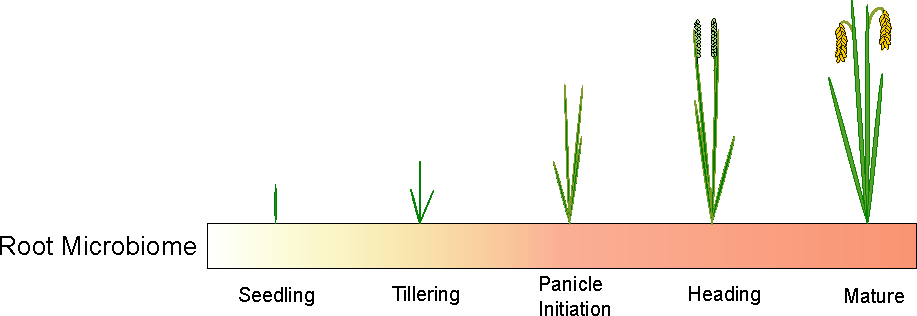
\includegraphics[width=5in]{Figures/figurec_3}
\caption[Figure 5.3]{\textbf{Model depicting the dynamic shifts in the microbiota over the course of a growing season as a function of plant developmental stage}}
\label{Figure 5.3}
\end{figure}

\section{Future Directions}
Here, I have described the composition, spatial structure, and acquisition of the rice root-associated microbiome, or the ``second genome'' of the plant. As I described earlier in this section, conceptual similarities exist between host-associated microbiota and genomes; however, it is unlikely that the similarities are limited to the examples above. Therefore, in moving forward with understanding the root-associated microbiota, it will be important for researchers to combine both ecological and genetic frameworks.

The functional impact of the microbiome as a whole on the host plant remains unknown. This is in large part because researchers have a lacked a controlled system to measure the traits of plants with and without a microbiota. This difficulty was overcome in animal systems by rearing germ-free mice (i.e. mice un-colonized by microbiota) which researchers could inoculate controlled microbial communities into and measure resulting traits \cite{Turnbaugh}. There is an ongoing effort by plant researchers with initial success to develop a similar axenic system to test how microbial consortia may impact plant traits (C. Santos, UC Davis, personal communication). 

To better understand how individual members of the root-associated microbiota impact plant fitness, an approach akin to ``mutagenesis'' could be used. Researchers are employing a relatively new approach to studying host-associated microbiota by introducing synthetic communities of cultured isolates to plant tissues \cite{bodenhausen2014synthetic,bai2015functional,lebeis2015salicylic}. It is conceivable that researchers could study the impact of a single microbial taxon on a given host trait by excluding it from an introduced synthetic community in a germ-free system, thus ``knocking out'' the microbe from the system. To extend this concept, a researcher could idenitify epistatic relationships between individual microbial taxa within a controlled system.

An alternative approach to discovering how individual microbial taxa affect plant host traits is by using an approach similar to a genome wide association study (GWAS). In GWAS, a genetic population with genotypic and phenotypic variation is used to correlate genetic variants (typically single nucleotide polymorphisms) with variation within phenotypic traits \cite{hardy2009genomewide}. Using this approach, it is possible to discover genes which may be responsible for a certain trait. One can imagine an example where a researcher can grow isogenic plants in different soils with sufficiently disparate microbiota to correlate the abundance of various microbes with plant traits. For example, if a researcher were to grow a single rice cultivar in 100 different salinity-stricken soils and measure the productivity of the plants, the researcher could correlate single microbial taxa or groups of taxa that may help plants survive under salt stress.

What result does microbiome hybridization have on the plant? In genetics, heterosis is a phenomenon where the resulting offspring of a genetic cross displays traits with better quality than either of the parents used to make the cross \cite{stuber1992identification}. If two soils with significantly different microbiota were to be mixed, would plants growing in the mixed soil display improved traits? If this were the case, could dominant and recessive microbes be identified that are responsible for the trait?

I hope I have made a persuasive case that using concepts derived from genetics as an approach for understanding root-associated microbiota provides a logical path forward with many interesting opportunities. The outcome will benefit not only researchers by accelerating progress in this field, but will be instrumental in unlocking the latent benefits of root-associated microbiota for crop growth and yield.
